\documentclass[a4paper,12pt]{article}
\setlength {\marginparwidth }{2cm}

% packages used
\usepackage{todonotes}
\usepackage{graphicx}
\usepackage{siunitx}
\usepackage{longtable}

% titlepage information
\title{ZRecognition\\TPJ665\\Final Capstone Project}
\author{Patrick Ziajski \\ Zarak Khattak}
\date{\today}

\begin{document}

% titlepage
\maketitle
\vfill
\begin{center}
    \textbf{SENECA COLLEGE OF APPLIED ARTS AND TECHNOLOGY}\\School of Electronics and Mechanical Engineering Technology\\1750 Finch Ave East, Toronto, Ontario, M2J 2X5. Tel. 416-491-5050\\www.senecacollege.ca
\end{center}
\thispagestyle{empty}
\pagenumbering{roman}

% table of contents
\newpage
\tableofcontents
\newpage
\listoffigures
\listoftables


% MAIN SECTION
\newpage
\pagenumbering{arabic}
\section{Executive Summary}
Z-Recognition is a License Plate Recognition system which provides clients with a new and intuitive way to implement and enforce parking systems. Our goal is to allow for the successful implementation of both hardware and software elements to allow for a working project.
The hardware aspect of the project involves the implementation of a microcontroller which will hold all the pre-required software to run the system. A camera that will be used to capture images of License plates. A speaker and a Servo Motor. 
The software aspect of the project entails the creation of a python script which will bring together all the hardware elements and have them operate with each other. The script will use the capture an image which will be processed as a JavaScript Object Notation (JSON) using Microsoft Azure Cognitive Services to process the image as text. The captured data will then be cross referenced against a database for validity and the Servo Motor will operate in response to valid data being found, whereas, the speaker will operate if no matching data is found.


% INTRODUCTION
\section{Introduction}
Security is an important feature for a company providing a service to their customer. The company must ensure that its service can only be used by authorized personnel. This is where Z-Recognition comes into play. Z-Recognition is a license plate recognition system that ensures only authorized personnel have access to a designated area. Z-Recognition accomplishes this by taking an image of the approaching vehicle and processing it. If the vehicle is authorized, meaning the license plate is recognized, the vehicle is given access. Our group has decided on a license plate recognition system due to its uses in modern day society. Today, one can still find areas that are monitored by a single employee, or by a ticket-based entry system. These systems could be found inferior because of their reliance on periodic human interaction or supervision. Z-Recognition is designed to run autonomously with minimal costs, and a single requirement of an active internet. This license plate recognition system also implements a core feature in the future of computer technology, machine learning. With machine learning, an artificial intelligence (AI) can provide systems the ability to learn and improve without being explicitly programmed. This means that automated systems become more secure and reliable, without the need of constant supervision. Finally, this project will require both hardware and software implementation to be fully functional. It will require us to work with and learn both software development and hardware assembly which we, as Computer Engineering and Technology students, would prefer.

\newpage
\section{Functional Features}
\begin{itemize}
    \item Image processing - Using Microsoft's Cloud based Computer Vision Service, called Azure, a captured image will be uploaded to Azure's Service. The service perform Optical Character Recognition (OCR) on the image, and it will return a JavaScript Object Notation (JSON) object with all the recognized characters.
    \item Motor Control - The Raspberry Pi 3 Model B, a MicroController Unit (MCU), will control a servo-motor to imitate a gate arm used to allow entrance into a secure area.
    \item Scheduled script execution - The main python script will be executed at specified time intervals
    \item Sound execution - The Raspberry Pi will emit a sound from a speaker in order to audibly notify the personnel using the system of whether they have been given or denied access.
\end{itemize}

\newpage
\section{System Specifications}
Camera
\begin{itemize}
    \item 720p/30fps
    \item Fixed focus
    \item Field of View - \ang{60}
\end{itemize}
Raspberry Pi 3 Model B
\begin{itemize}
    \item Quad Core 1.2GHz Broadcom BCM2837 64bit CPU
    \item 1GB RAM
    \item BCM43438 wireless LAN
    \item 40-pin extended GPIO
    \item 4 Pole stereo output
    \item Micro SD
\end{itemize}
Servo-motor
\begin{itemize}
    \item Operating voltage - 3.0V ~ 7.2V
\end{itemize}
Microsoft Azure
\begin{itemize}
    \item Active subscription
    \item Cognitive Services resource
\end{itemize}

\newpage
%OPERATING INSTRUCTIONS
\section{Operating Instructions}

Please follow the listed steps to ensure that the system is operating as intended:

\begin{itemize}
    \item Ensure that the Raspberry Pi Microprocessor is powered on
    \begin{itemize}
        \item Plug the power cord into the Pi and connect to a power source
        \item Launch the python script
    \end{itemize}
    \item Connect the Pi to an internet source
    \begin{itemize}
        \item Connect using Wi-Fi or using an Ethernet Cable
    \end{itemize}
    \item Ensure that the Camera is on
    \begin{itemize}
        \item Connect the Camera to a powersource and aim in the direction towards which you want to capture the images
    \end{itemize}
\end{itemize}


\section{Product Design, Implementation, and Operation of the System}

\subsection{System Block-Diagram}
\begin{figure}[ht]
    \centering
    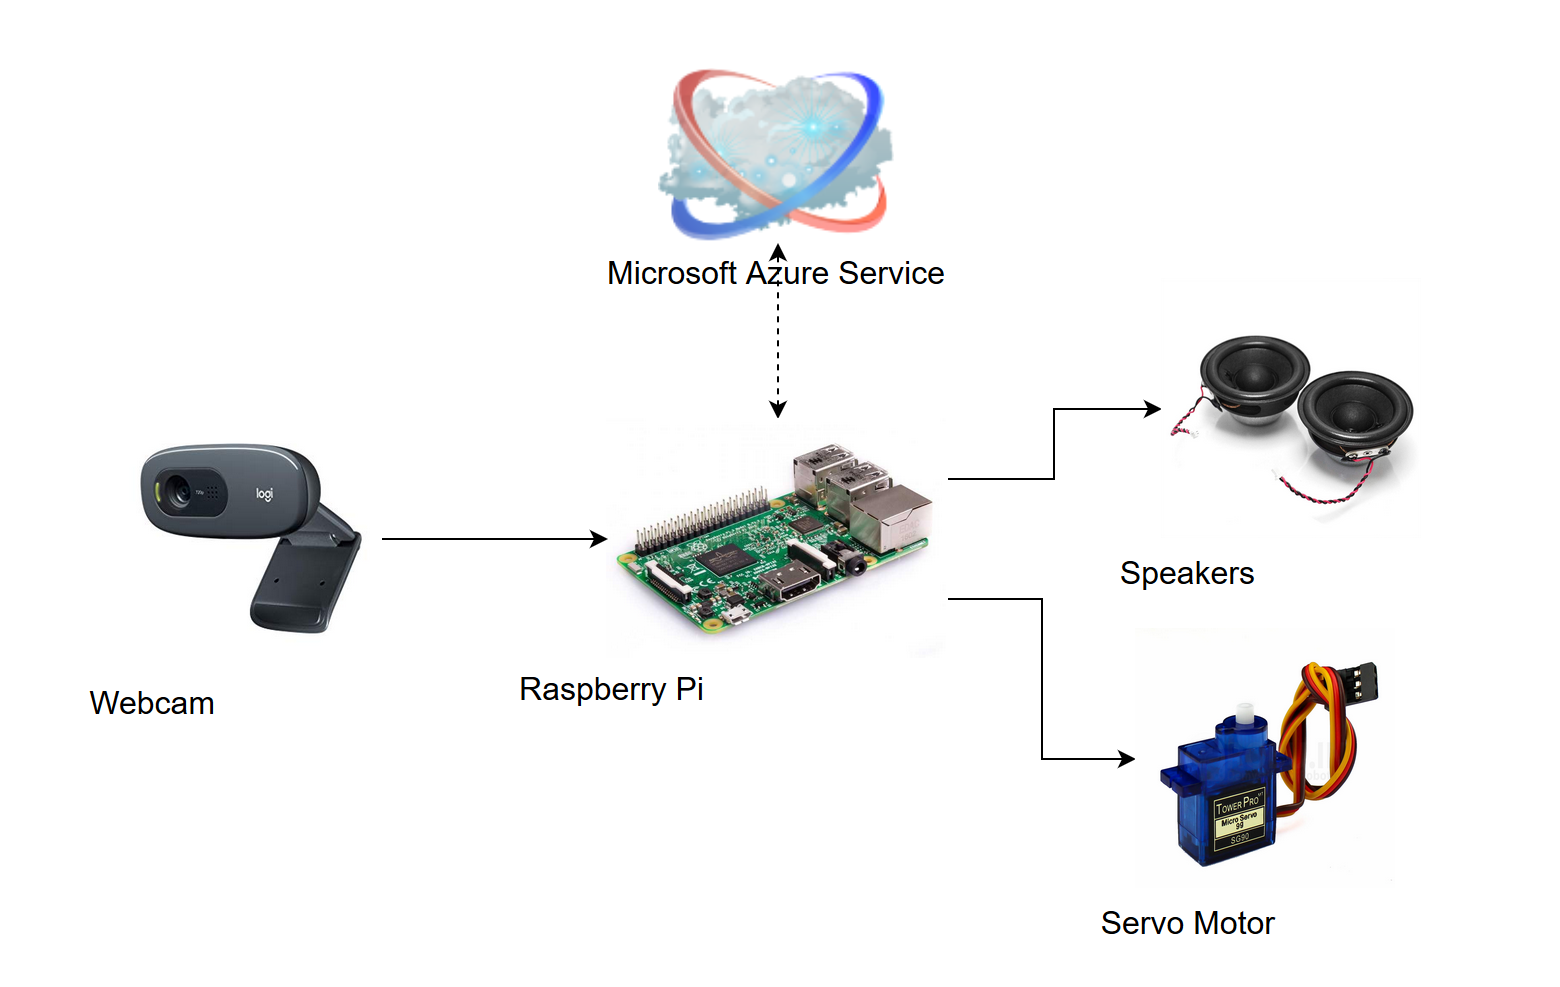
\includegraphics[width = \linewidth]{../images/BlockDiagram.png}
    
    \caption{System Block-Diagram}
\end{figure}

\subsection{UML Diagram}
\subsection{Software Flow-Chart}

\subsection{Component images and components description/Captures of the major GUI used}

The system utilized in this project consists of a few major components. Each component is listed and described below:

\begin{itemize}
\item Microprocessor - Raspberry Pi 3 Model B
\begin{itemize}
    \item The Raspberry Pi 3 Model B will act as the sole microprocessor for this project. It is programmed with a python script that is executed to run the program. The Pi makes use of  a 1.2GHz Quad Core 64bit CPU with 1GB built in RAM.
\end{itemize} 
\item Camera - Logitech C270 HD Webcam
\begin{itemize}
    \item The Logitech C270 Webcam is installed to ensure that the images captured are of high quality so that they are easy to interprit. These Images are taken in 720p with a fixed focus and field of view of \ang{60} These images are interpreted by the Microsoft Azure Cognitive services and returned back as a JSON object.
\end{itemize}
\item Servo Motor
\begin{itemize}
    \item The RioRand SG90 Micro 9d Servo motor will be the sole motor that will be utilized. 
\end{itemize}
\end{itemize}

\subsection{Theory of operation of the entire system}

% APPENDIX
\newpage
\section{Maintenance Requirements}

Routine maintenance is a good way to avoid any unwanted interruptions for the services being provided. It is recommended that proactive maintenance be done on the system at a frequency of one week (7 days) or anytime that the system fails to operate.
\\
\\
    • Reset the Pi Microprocessor
\\
    •	Relaunch the Python script
\\
\\
Please ensure that you test the service after completing maintenance to ensure that all systems are up and running. 

If you are unsure of how to complete any of these tasks, please get in touch with the contacts available in the contact(s) section of the report.

\appendix
\section{Electrical Schematics}

\section{Parts List}

\begin{longtable}[c]{| l | c | c |}
    \hline
    \multicolumn{3}{| c |}{\textbf{BILL OF MATERIALS}}\\
    \hline

    \textbf{Component Name} & \textbf{Quantity}  & \textbf{Price (CAD)} \\
    \hline
    Raspberry Pi 3 Model B & 1 & \$35.00 \\
    \hline
    Logitech C270 HD Webcam & 1 & \$32.00\\
    \hline
    RioRand 5PCS x SG90 Micro 9d Servo & 1 & \$16.99\\
    \hline
    Gikfun 2" 8 Ohm 2W Audio Speaker & 1 & \$16.88\\
    \hline
    \multicolumn{2}{|l|}{\textbf{Total Cost w/ Tax}} & \$113.98\\
    \hline

    \caption{Bill of Materials}\\

\end{longtable}
*NOTE* All prices are in Canadian Dollars (CAD)

\section{List of all User Names and passwords used in software}
Currently there are no log in credentials required for any aspect of the software system
\section{References}

\newpage
\section{Contact Information}
\begin{center}
    Patrick Ziajski \\*
    Phone: (647) 339 2847 \\*
    Email: pziajski@myseneca.ca \\
    \vspace{5mm}
    Zarak Khattak \\*
    Phone: (587) 226 3196\\*
    Email: zkhattak@myseneca.ca
\end{center}

% \section{Description of the attached CD content}

\end{document}